\documentclass[conference]{IEEEtran}
\IEEEoverridecommandlockouts
% The preceding line is only needed to identify funding in the first footnote. If that is unneeded, please comment it out.
\usepackage[utf8]{inputenc}
\usepackage[T1]{fontenc}
\usepackage{cite}
\usepackage{amsmath,amssymb,amsfonts}
\usepackage{algorithmic}
\usepackage{graphicx}
\usepackage{textcomp}
\usepackage{xcolor}
\usepackage{hyperref}
\def\BibTeX{{\rm B\kern-.05em{\sc i\kern-.025em b}\kern-.08em
    T\kern-.1667em\lower.7ex\hbox{E}\kern-.125emX}}
\begin{document}

\title{Dot Matrix Notifier}

\author{\IEEEauthorblockN{Daniel Hipp}
\IEEEauthorblockA{\textit{Faculty of Computer Science} \\
\textit{HTWG Konstanz}\\
Konstanz, Germany\\
dahipp@htwg-konstanz.de}
\and
\IEEEauthorblockN{Etienne Gramlich}
\IEEEauthorblockA{\textit{Faculty of Computer Science} \\
\textit{HTWG Konstanz}\\
Gailingen, Germany\\
etgramli@htwg-konstanz.de}
\and
\IEEEauthorblockN{Thomas Gnädig}
\IEEEauthorblockA{\textit{Faculty of Computer Science} \\
\textit{HTWG Konstanz}\\
Singen, Germany \\
thomas.gnaedig@htwg-konstanz.de}
}

\maketitle

\begin{abstract}
ToDo
\end{abstract}


\begin{IEEEkeywords}
LED, dot matrix, LED matrix, Android, smartphone, WiFi, notification
\end{IEEEkeywords}


\section{Introduction}
The goal of this project is to provide a screen that show notifications and text from a smartphone so that they are better visible. It should stand alone somewhere in the room and is not intended as an extension to smartphone itself. The next step is to provide image thumbnails on the screeen.

An inexpensive replacement for a screen is a dot matrix, that consists of a rectangular array of LEDs. Such a dot matrix can be easily connected to an Arduino or Raspberry Pi. Due to the networking requirement of the task a Raspberry Pi version 3 seems to be the better choice over an Arduino. The latest Raspberry Pi has multiple network interfaces, such as LAN, WiFi and Bluetooth.


\section{State of the Art}
In this chapter we name three diffrent Products with similar behavior as our Matrix.

First of all there is the TEBE \cite{ledtebe}, this Matrix has only one row for letters wich can be infinite long. Our Matrix got only one row too, but the length is limited by 16 LEDs. In contrast to our Matrix, there is the possibility to use multiple Color for the LEDs, colored text can be shown if needed, but no support for colored images is avaliable. To print some Letters on the TEBE Matrix, you need to use a windows application and set your text. Special characters like Stars are supported, but no image can be shown. Compared with our Matrix we just need a Smartphone to change the currently displaying message. So the TEBE is more suitable for static outputs, wich have only to be changed a few times a day. There is a timemanaging system, were you can define, how often your message should change, but you need to know this message at initialisation time. Therefore this module can be used inside and outside. Our Matrix is just suitable for dry environments. An extension to the TEBE Matrix is the Proline \cite{ledproline}. This serie supports multiple lines above, in theory there is no limitation for the number of rows to be used. But there is still no imagesupport as in our Matrix avaliable. It is possible to Print out different Characters on different rows with individual color, so you could try to do some ASCII-Arts but no real image can be shown.

Another comparable product is the Eurolite ESN \cite{esn}. There is also just one row of Characters possible. Therefore each Pixel can be shown in different color. The output can be displayed in 14 different fonts, is able to blink if necessary and can move to any direction. Out Matrix just supports one direction and only one font with capital Letters and some special characters. Another nice Feature is that the current time can be displayed in different styles (DD.MM.YYYY, US/UK or MM.DD.YYYY). This feature could be implemented to our matrix in future work. Even though there is the possibility to color each LED separately, there is still no image support avaliable.


\section{Proposed approach}
Since our dot matrix should sit somewhere in the room, it must connect wirelessly to the user's smartphone. As smartphones usually have WiFi and Bluetooth interfaces built-in and do not contain a LAN interface, WiFi and Bluetooth are the intersection of both devices.

As with web servers threre are already well-established technologies, we decided to transfer our application's data over HTTP from the client to the server. We will programm an Android app, so that the user can easily interact with our matrix. The implementation approach is discussed in the following sections.


\subsection{Coose the matrix}
The matrix must be compatible with the Rasbperry Pi, but for testing purposes the compatibility to Arduino is desirable. So the protocol must be either SPI or I\textsuperscript{2}C, because both are supported on Raspberry Pi and Arduino.

It also must not consume more energy than the Raspbery Pi and Arduiono can provide, that makes it more easy to assemble and run. So it must work at a volate of 3.3V or 5V and must draw at most 50mA and 300mA repectively~\cite{rpiperipherals}.

Since there are no square, pre-assembled matrices of a size of 16x16 or larger, we have to build one out of smaller dot matrices. So the individual matrix must be addressable individually. So that a wrapper library can be built that acts as a sinle panel and outputs part of the image on the respective sub-matrix.

There are models with various sizes using the MAX7219 chip, which is an IC display driver for dot matrices and 7-segment LED displays. It makes programming in Python very easy and is compatible with both Arduino and Raspberry Pi.

\subsection{Communication between Raspberry Pi and the matrix}
The communication interface between the Raspberry Pi and the matrix must support multiple connection, so that multiple matrices can be combined to one larger matrix. For example SPI supports multiple slaves (matrices) that would be connected to one master (the Raspberry Pi). Also I\textsuperscript{2}C supports multiple slaves by different addresses and even multiple masters, the latter is not important for our use case.

In our setup, we use two 8x16 LED-Matrices, wich are created by two combined 8x8 Matrices. The comminuication is completely handeled my the MAX7219 and we can see them as one 8x16 Matrix. To connect both 8x16 Matrices in parallel to the same output at the Pi, they need to get different adresses.
After the basic setup is done, we created a python module wich handles the two different Matreices as one 16x16 Matrix. This can be done by splitting the input into half and send the upper informations to the first- and the other part to the secound adress. This comminication is done by the Adafruit\_LED\_Backpack\cite{ledlibrary} library, wich takes a 8x16 shaped array and sends it to the defined adress at the I\textsuperscript{2}C bus.

To display messages, the incoming string has to be converted into something wich fits on our 16x16 Matrix. Therefor we choose a font to convert each incoming char to a 8x$n$ array, the $n$ is depending on the char value. The $n$ lies betwen two, for a dot, and six for the uppercase letter M. The complete representation of an incoming string is a concatenation of all arrays from the converted chars, so the resulting shape is 8x$N$. To display this representation on our 16x16 Matrix, the shape has to be adjusted. This can be done by adding zero padding above and below the representation, so the Result is a 16x$N$ array, with letters in rows five to twelve and zeros in the other rows. Now we can display a 16x16 shaped submatrix of the full representation by indexing. The selected columns are increased sequentially with a short delay, in our case 0.125 sec, and displayed to the LED-Matrix. To get a smooth transition between the Incoming Text and the empty Matrix, we also concatenate a 16x16 zero array before and after the representation.
To Display an binary image, we just convert the incoming string to an binary 16x16 array.

\subsection{Communication between the Client and Server}
Since WiFi and Bluetooth is the intersection of the Raspberry Pi's and smartphone's network interfaces, the communication must use one of those. Because the user may already have the smartphone connected to a headphone or headset, we chose to use the smartphone's Wifi interface. But to maintain normal smartphone usage, the internet connection that was previously possible by the user's WiFi, the Raspberry Pi must be connected to the internet via LAN and act as an access point for the smartpone. This way we can ensure that the Raspberry Pi has an static IP address, making the connection easier. Figure~\ref{FIG:COMMUNICATION} shows an overview of the network connection. The communication between the smartphone App and the Pi is done by simple running a HTTP server on the Pi. To send data to the Matrix, the App just has to send an HTTP-GET request. The requested Page is not a real Page, it has to be the Message or Picture wich should be shown on the Matrix. To distinguish between a text and a image we defined a capital letter for both types. to send a text to the Pi, the get request has to look like this : GET /S\textit{text\_to\_display} for an image the letter I has to be used. Because the Matrix supports only on and off and no colors or brightnesses the image data is just made of ones and zeros. To representate the image as string it has to be converted to a 16x16 binary image. This has to be converted to a 16x16 binary array by using a threshold. Now the array has to be flattened and the result should be a vector with 256 entries, each can either be one or zero. to display this flattened image the get request should look like this : GET /I\textit{011010110...}. Whenever the server on the pi gets an HTTP-GET request, a method is called, to check if its a legal request and then interprets the payload as image or string, depending on the first letter.

\begin{figure}[ht]
\label{FIG:COMMUNICATION}
\centering
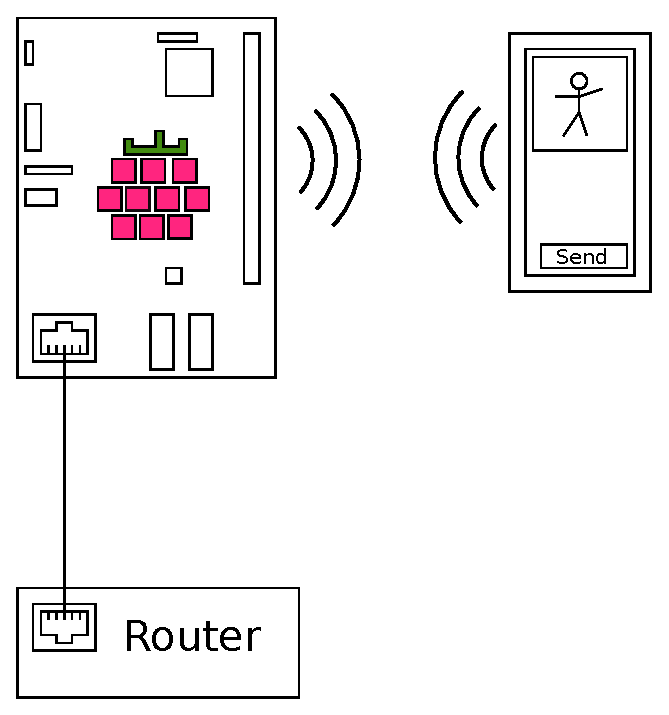
\includegraphics[width=0.75\linewidth]{pics/RasPi-MC}
\caption{Communication overview between Raspberry Pi, Smartphone and Router}
\end{figure}

To send text and images from the smartphone to the Raspberry Pi, we use HTTP requests containing the text itself (with escaped special characters), or the image encoded as '0's and '1's in a binary image.

\subsection{WiFi access point}
To function as an access point, the Raspberry Pi needs packages for the access point itself, a DHCP server and for network address translation (NAT). Therefore two daemons are needed, one for using the WiFi interface as an host for the access point (hostapd) and one DHCP daemon.

The host access point daemon is configured to use the Raspberry Pi's built-in WiFi chip as the network interface and WPA2  encryption with a predefined password.

The DHCP server must assign an address to the smartphone connecting to the WiFi. It also communicates the Raspberry Pi as the Gateway so that the smartphone can connect to the internet.

Iptables is configured so that the smartphone in the Raspberry Pi's WiFi can access the internet through NAT at the Pi's LAN interface. This is solved that way, that new connections from the WiFi are accepted, but no new connections from the LAN NIC. Packages at the LAN NIC are only accepted, when they belong to an existing connection.


\section{Results}
Finally we use a Raspberry Pi to drive two dot matrices and act as an access point for the smartphone. It routes normal internet traffic through its LAN interface to the existing router. The detailed description of our solutions follows in this chapter.

\subsection{Difficulties}
Difficulties arose from the first matrix that we used. It was a 8x32 controlled by a MAX7219 chip~\cite{azdelivery464}, that was supposed to work with both Arduino and Raspberry Pi. Not even the example code from the manufacturer's repository~\cite{azdelivery464} worked on our Raspberry Pi 3, the matrix only printed random looking patterns. Neither a level shifter from 5V to 3.3V nor a separate power supply for the dot matrix did solve the problem. Therefore we moved to dot matrices from Adafruit~\cite{adafruit88}. That new matrix worked flawlessly with the Raspberry Pi, and has a ``backpack'' with an I²C interface, instead of SPI.

\subsection{Communication}
The Raspberry Pi is our connection hub and main device. It has to connect the smartphone to the matrix and so has to maintain connection to both. The Raspberry Pi also delivers the power for the matrix from its own power supply.

\subsection{Communication between the Client and Server}
The communication between the server software on the Raspberry Pi and the client on the smartphone is done with HTTP requests. Only strings can be sent to the Raspberry Pi, so images gave to be encoded as strings.

If the received strings only contains zeroes and is 256 (16x16) numbers long, it will be interpreted as an binary image and directly outputted on the dot matrix.

If the message contains also other ASCII characters, it will be interpreted as a string. Special characters (i.e. apersand, space) must be escaped before sending to the Raspberry Pi. The characters are converted with a special font to images and outputted on the matrix.

\subsection{Communication between Raspberry Pi and the matrix}
We use two 8x16 matrices above each other to form a large 16x16 matrix. Both are connected as slaves to the Raspberry Pi's I\textsuperscript{2}C interface. Therefore the two matrices need different addresses, so one of the matrices needs to be soldered to alter its default address.

After that step both matrices can be used at the same I\textsuperscript{2}C interface at the Raspberry Pi. But since there are only python libraries for one 8x16 matrix, we wrote a wrapper so that both matrices appear as a single 16x16 matrix. So we can print images on the matrix, to write text on the matrix one needs a special font for low resultion screen. With that we can render the glyphs of the text and display them on the matrix. For long texts we implemented scrolling from right to left.

\subsection{The Android App}
After the user installed the app he is able to send a text or an image to the dot matrix. Additionally the app sends the icons of incoming notifications to the matrix. To achieve this, the app sends a http-request to the Rapsberry Pi with the text or image enbedded into the request. The requests are sended with the help from vollay, an Android library to send messages between multiple endpoints. The bitmaps of the images to be sent are scaled in size to 16x16 pixels and are converted to black-white binary images. At last they are changed into a string to make sendig over a HTTP request possible. The last point is the notification service which sends the notification's icon, which gets converted as normal images. The notification-service can be turned off by the user. Finally the user can use our app to show his favorit texts and images or notifications on a matrix. Figure~\ref{FIG:APP} shows the home screen of our app, leading to the options to send text and images.

\begin{figure}[ht]
\label{FIG:APP}
\centering
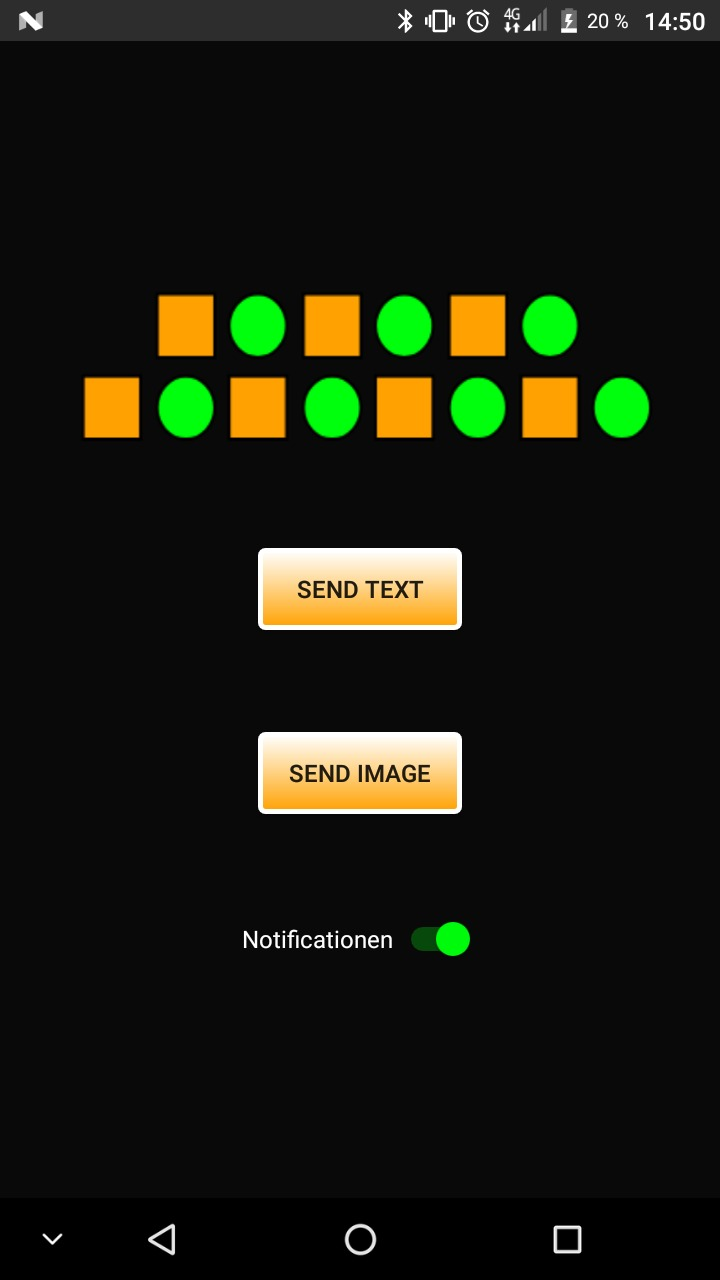
\includegraphics[width=0.75\linewidth]{pics/AppHomeScreen}
\caption{Home screen of our Android app}
\end{figure}


\section{Conclusion}



\section{Further Work}
There are some parts in our project, that can be improved or further developed. The most important ideas will be discusst in the following sections.

\subsection{Dot Matrix}
Improvements can be made with better matrices, for example multi-color matrices or those that can be dimmed, to display a color image or a greyscale image respectively. A bigger matrix is possible, too. All this needs more computing power, but the Raspberry Pi is easily capable of this task, but an Arduino might not capable of that. The replacement of the matrix makes changes to the wrapper inevitable and one has to consider the power consumption of a larger matrix, a 32x32 dot matrix might draw up to 4A at 5V.

As new Feature a clock could be implemented, wich shows the current time, whenever no requests are incoming. So it could be used as simple clock even without a smartphone connected.

\subsection{Server Security}
Since the web server is not secured, multiple smartphones can connect to the Raspberry Pi and all of them can send messages to the Raspberry Pi simulateously. One possibility is that only one smartphone should be able to connect to the server. It can be achieved by a code, that is displayed on the matrix and entered on the smartphone. This makes sure that only the first smartphone is able to send messages. Optionally an encryptet HTTP connection could be used, to make the messages not readable for third parties.


%%--- Write text above here, all references below here ---%%
\begin{thebibliography}{00}
\bibitem{ledtebe}
  ACT GmbH,
  ``Laufschrift Serie TEBE''.
\bibitem{ledproline}
  ACT GmbH,
  ``Laufschrift Serie Proline''.
\bibitem{esn}
  eurolite,
  ``ESN 7x80 5mm LED-Laufschrift''.
\bibitem{rpiperipherals}
  Elinux.org,
  ``RPi Low-level peripherals'',
  \url{https://elinux.org/Rpi_Low-level_peripherals#General_Purpose_Input.2FOutput_.28GPIO.29},
  2019.
\bibitem{azdelivery464}
  AZ-Delivery,
  ``4 x 64er LED Matrix Display'',
  \url{https://www.az-delivery.de/products/4-x-64er-led-matrix-display?ls=de},
  12. 01. 2019.
\bibitem{adafruit88}
  Adafruit,
  ``Adafruit Mini 8x8 LED Matrix w/I2C Backpack - Yellow'',
  \url{https://www.adafruit.com/product/870},
  12. 01. 2019.
\bibitem{adafruit3232}
  Adafruit,
  ``32x32 RGB LED Matrix Panel - 6mm pitch'',
  \url{https://www.adafruit.com/product/1484},
  15. 01. 2019.
\bibitem{ledlibrary}
  Adafruit,
  ``Adafruit Python LED Backpack'',
  \url{https://github.com/adafruit/Adafruit_Python_LED_Backpack},
  14. 01. 2019.
\end{thebibliography}
\end{document}
